\problemname{Chess}
%{Daniel Brinkers}{1}
In chess the bishop is the chessman, which can only move diagonal. It is well
known that bishops can reach only fields of one color but all of them in some
number of moves (assuming no other figures are on the field). You are given two
coordinates on a chess-field and should determine, if a bishop can reach the
one field from the other and how. Coordinates in chess are given by a letter
('A' to 'H') and a number (1 to 8). The letter specifies the column, the number
the row on the chessboard.

%figure
\begin{figure}[h]
	\centering
	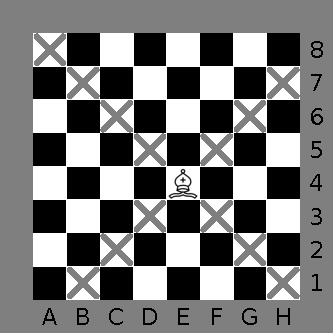
\includegraphics[width=0.6\textwidth]{images/chess.pdf}
	\caption{Chessboard, bishop and fields the bishop can reach in one move}
\end{figure}

\section*{Input}
The input starts with the number of test cases. Each test case consists of one
line, containing the start position $X$ and end position $Y$. Each position is
given by two space separated characters. A letter for the column and a number
for the row. There are no duplicate test cases in one input.

\section*{Output}
Output one line for every test case. If it's not possible to move a bishop from
$X$ to $Y$ in any number of moves output '{\tt Impossible}'. Otherwise output one possible
move sequence from $X$ to $Y$. Output the number $n$ of moves first (allowed to be
$4$ at most). Followed by $n + 1$ positions, which describe the path the bishop
has to go. Every character is separated by one space. There are many possible
solutions. Any with at most $4$ moves will be accepted. Remember that in a chess
move one chessman (the bishop in this case) has to change his position to be a
valid move (i.e.\ two consecutive positions in the output must differ).
